\documentclass{article}
\usepackage[utf8]{inputenc}
\usepackage[margin=0.75in]{geometry}
\usepackage{enumerate}
\usepackage{amsmath}
\usepackage{amsfonts} 
\usepackage{amssymb}
\usepackage{amsthm}
\usepackage{mathtools}
\usepackage{float}
\usepackage{array}
\usepackage{makecell}
\usepackage{commath}
\usepackage{verbatim}

\DeclarePairedDelimiter{\ceil}{\lceil}{\rceil}

\renewcommand\theadalign{bc}
\renewcommand\theadfont{\bfseries}
\renewcommand\theadgape{\Gape[4pt]}
\renewcommand\cellgape{\Gape[4pt]}

\newcommand{\N}{\mathbb{N}}
\newcommand{\Z}{\mathbb{Z}}
\newcommand{\Q}{\mathbb{Q}}
\newcommand{\C}{\mathbb{C}}
\newcommand{\R}{\mathbb{R}}
\newcommand{\F}{\mathbb{F}}
\newtheorem{theorem}{Theorem}
\newtheorem{corollary}{Corollary}[theorem]
\newtheorem{definition}{Definition}[theorem]
\newtheorem{lemma}[theorem]{Lemma}
\newtheorem*{remark}{Remark}
\newcommand{\cdotscalar}{\;\widetilde{\cdot}\;}
\newcommand{\vectorplus}{\;\widetilde{+}\;}
\newcommand{\Span}{\text{Span}}
\newcommand{\Null}{\text{Null}}
\newcommand{\Range}{\text{Range}}
\newcommand{\D}{\frac{d}{\dif x}}

\renewcommand{\epsilon}{\varepsilon}
\renewcommand{\phi}{\varphi}

\newcommand{\Or}{\mbox{ OR }}
\renewcommand{\And}{\mbox{ AND }}
\newcommand{\Not}{\mbox{NOT }}
\newcommand{\Iff}{\mbox{ IFF }}

\newcommand{\Width}{\textup{width}}
\newcommand{\Mesh}{\textup{mesh}}
\newcommand{\Int}{\textup{Int}}
\newcommand{\Ext}{\textup{Ext}}
\newcommand{\Bd}{\textup{Bd}}


\newcommand\widebar[1]{\mathop{\overline{#1}}}
\newcommand*\closure[1]{\widebar{#1}}

\newcommand\Ball[2]{U(#1; #2)}

\begin{document}

\section*{Question 2: Feature Maps}

\begin{enumerate}[(a)]
    \item This data is not seperable by a linear classifier. We know that a linear classifier separating this data must partition $\R^2$ into half-spaces $H_1$ (positive) and $H_0$ (negative) based on a threshold $t$. 
    
    In this dataset, $p_1 = (-2, -1)$ and $p_2 = (2, 3)$ have label $1$, and so are in $H_1$. We know that half-spaces are convex, and so any convex combination of $p_1$ and $p_2$ must lie in $H_1$. If we take $\lambda = 3/4$, then 

    \[p_2 = p_1 + \lambda(p_2 - p_1) = (-2, -1) + \frac{3}{4}(2 - (-2), 3 - (-1)) = (-2, -1) + \frac{3}{4}(4, 4) = (1, 2)\]

    must lie in $H_1$ since it is convex combination of $p_1$ and $p_2$. However, we know that $p_3$ has label $0$, and so must lie in $H_0$. This is a contradiction, and so no linear classifier can separate this data.
    \item We will assume that a threshold $t = 0$ is used. The constraints are as follows:
    
    \begin{align}
        -2w_1 + w_2 &\geq 0\\
        w_1 + 4 w_2 &< 0\\
        2w_1 + 9w_2 &\geq 0
    \end{align}
    \item The feasible area is given by the intersection of the blue, red, and green half-spaces below, which is the shaded region to the left of the red line, above the green line, and below the blue line. The feasible area is shown in Figure \ref{fig:q2c}.
    
    \begin{figure}[H]
        \centering
        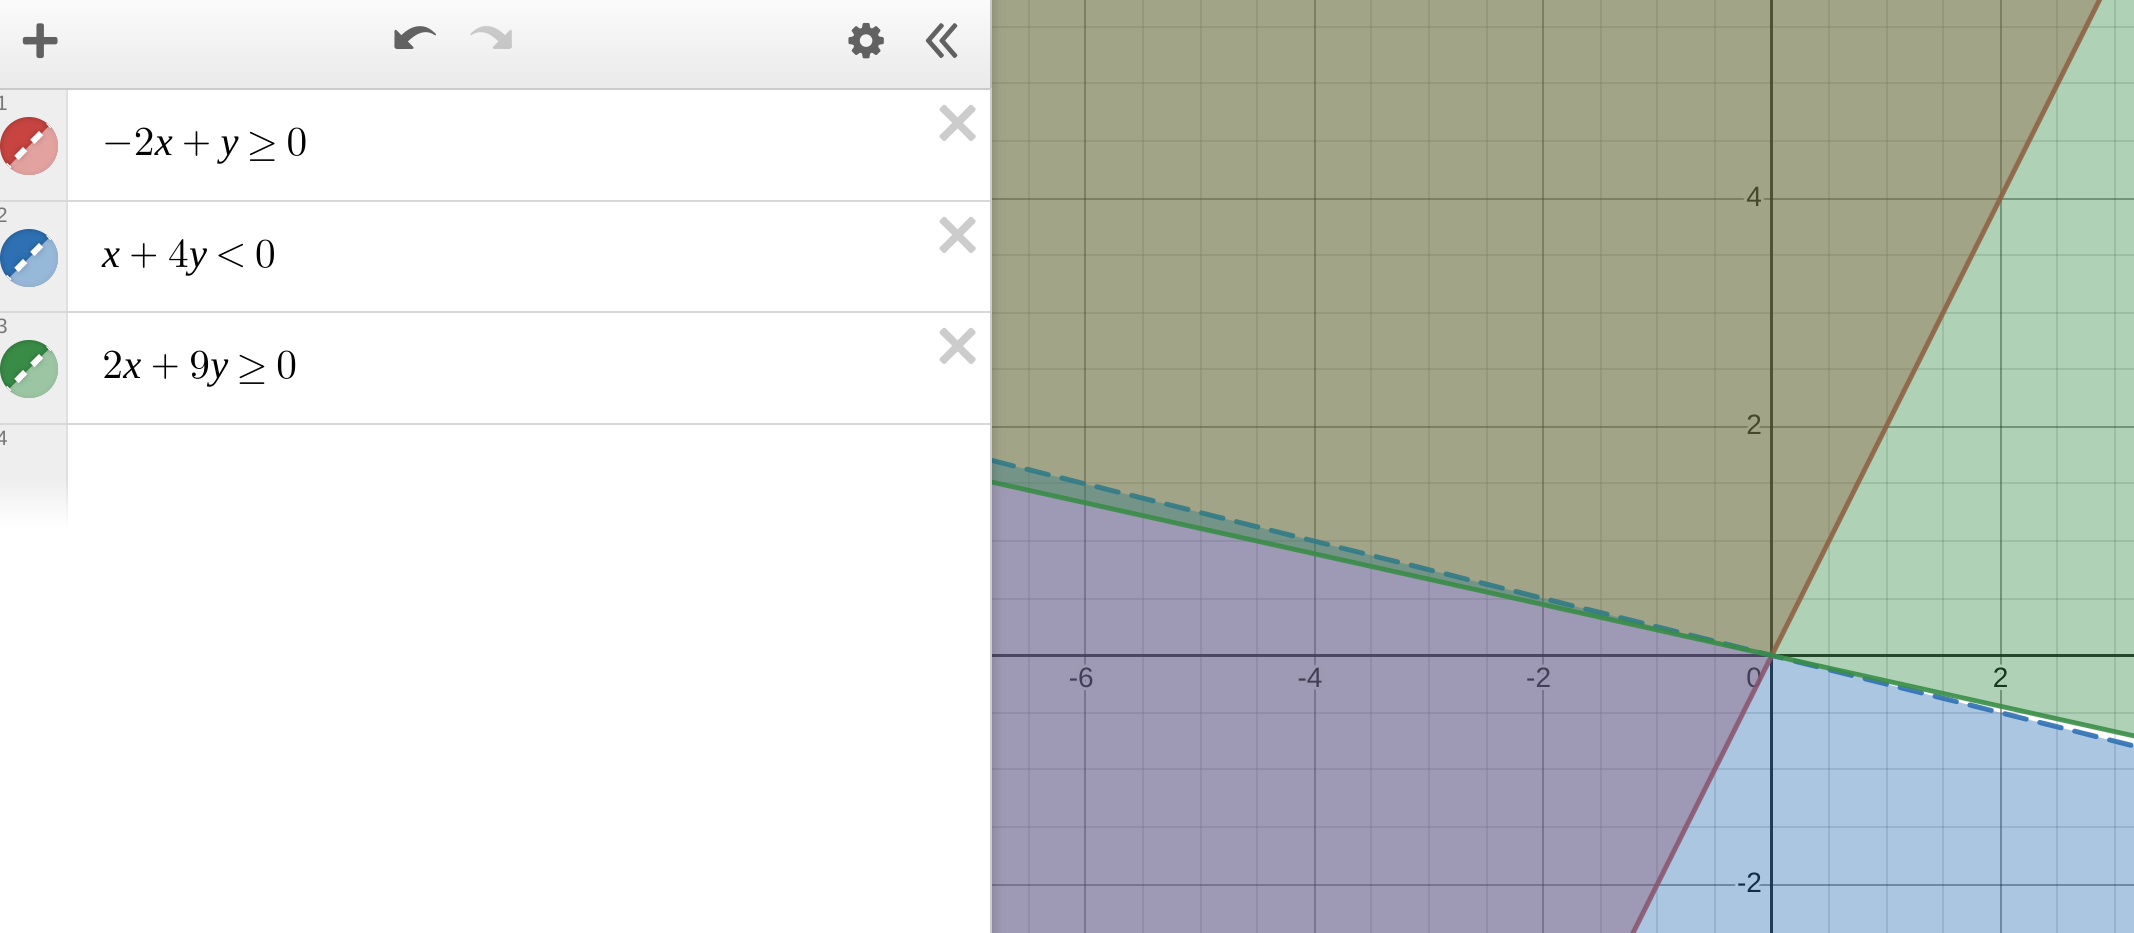
\includegraphics[width=0.9\textwidth]{../figures/q2_c_feasible_area.png}
        \caption{Feasible area for $w_1, w_2$}
        \label{fig:q2c}
    \end{figure}
\end{enumerate}

\newpage
\section*{Question 3: kNN vs Logistic Regression}

\begin{enumerate}[(a)]
    \item The plot of classification vs validation accuracy is given below in Figure \ref{fig:q3a}.
    
    \begin{figure}[H]
        \centering
        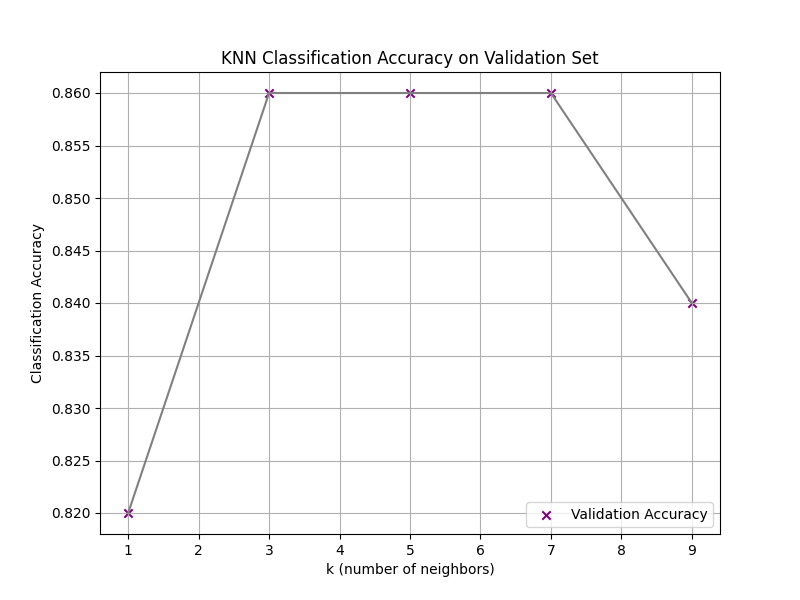
\includegraphics[width=0.7\textwidth]{../figures/knn_classification_accuracy.png}
        \caption{Classification vs Validation Accuracy}
        \label{fig:q3a}
    \end{figure}

    \item The value of $k^*$ chosen is $k^* = 3$. This is because $3$ is the smallest value of the hyperparameter $k$ which achieves the maximum accuracy seen across all values of $k$ (0.860). I have chosen this value of $k$ in adherence with the principle of Occam's Razor, which states that the simplest solution is often the best one. In this case, the simplest solution is the least complex model (lowest $k$), as the model complexity increases with $k$. 
    
    Here is a report of the validation and test accuracies for $k^*, k^* + 2, k^* - 2$:

    \begin{verbatim}
        Classification accuracies for k_star=3
            Validation accuracy: 0.86
            Test accuracy: 0.92
        Classification accuracies for (k_star + 2)=5
            Validation accuracy: 0.86
            Test accuracy: 0.94
        Classification accuracies for (k_star - 2)=1
            Validation accuracy: 0.82
            Test accuracy: 0.88
    \end{verbatim}

    We see that the maximum validation accuracy is reached when $k^* = 3$, increasing from 0.82 when $k = 1$ and staying at the same value of 0.86 when $k = 5$.
    
    However, the test accuracy increases from $0.88$ to $0.92$ when going from $k^* - 2$ to $k^*$, and continues to increase with $k = k^* + 2 = 5$. This illustrates that the simplest model that performs best on the validation set may not always be the one that performs best on the test set. 
\end{enumerate}

\end{document}